\chapter{Экспериментальный раздел}
В текущем разделе будет поставлена цель эксперимента, проведён сам эксперимент и сделаны соответствующие выводы. 

\section{Технические характеристики}

Технические характеристики устройства, на котором выполнялось тестирование, следующие.

\begin{itemize}
	\item Операционная система: Windows 10 \cite{oswind} x86\_64.
	\item Память: 8 GiB.
	\item Процессор: 11th Gen Intel® Core™ i5-1135G7 @ 2.40GHz \cite{intel}.
	\item 4 физических ядра и 8 логических ядра.
\end{itemize}

Тестирование проводилось на ноутбуке, включенном в сеть электропитания. Во время тестирования ноутбук был нагружен только встроенными приложениями окружения, а также непосредственно системой тестирования.


\section{Постановка эксперимента} 

\subsection{Цель эксперимента}
Целью эксперимента -- оценка оптимизированного алгоритм обратной трассировки лучей для данной сцены. 

Время отрисовки сцены напрямую зависит от количества лучей. Оптимизация, представленная в данной работе, направлена на уменьшение количества лучей, что в свою очередь позволит уменьшить время. 

Для подтверждения данной гипотезы необходимо провести теоретическое сравнение оптимизированного и неоптимизированного алгоритма, а также подтвердить результаты на практике путем подсчета количесва испускаемых лучей для построения сцены.

%Эксперимент будет проводиться на различных сценах, с разным количеством этажей дома, а также с разными видами молнии.
%\begin{enumerate}
%	\item Количество этажей -- 6, молния без побочных ветвей бьет в громоотвод, количество окон, в которых горит цвет -- не имеет значения.
%	\item Количество этажей -- максимальное, молния-лидер с большим количеством ветвей бьет в землю, во всех окнах не горит свет.
%	\item Количество этажей -- минимальное, молния без ветвей бьет в громоотвод, во всех окнах горит свет. 
%	\item Количество этажей -- 5, молния-лидер бьет в землю, количество окон, в которых горит свет -- не имеет значение.
%	\item Количество этажей -- максимальное, молния-лидер бьет в землю, во всех окнах горит свет.
%\end{enumerate}

%Также будет приведены:
%\begin{itemize}
%	\item график зависимости количества испускаемых лучей от количества окон, в которых не горит свет (учитываются только те окна, которые  ''видны'' пользователю);\\
	
%	\item график зависимости времени построения от количества окон, в которых не горит свет.
%\end{itemize}


\subsection{Теоретическое сравнение алгоритма обратной трассировки лучей}

\subsubsection{Рассчет количества лучей}

\textbf{Описание}: Количество этажей -- 5, молния без побочных ветвей бьет в громоотвод, во всех окнах выключен свет.

Результат представлен на рисунке \ref{img:s1}.
\begin{figure}[H]
	\begin{center}
		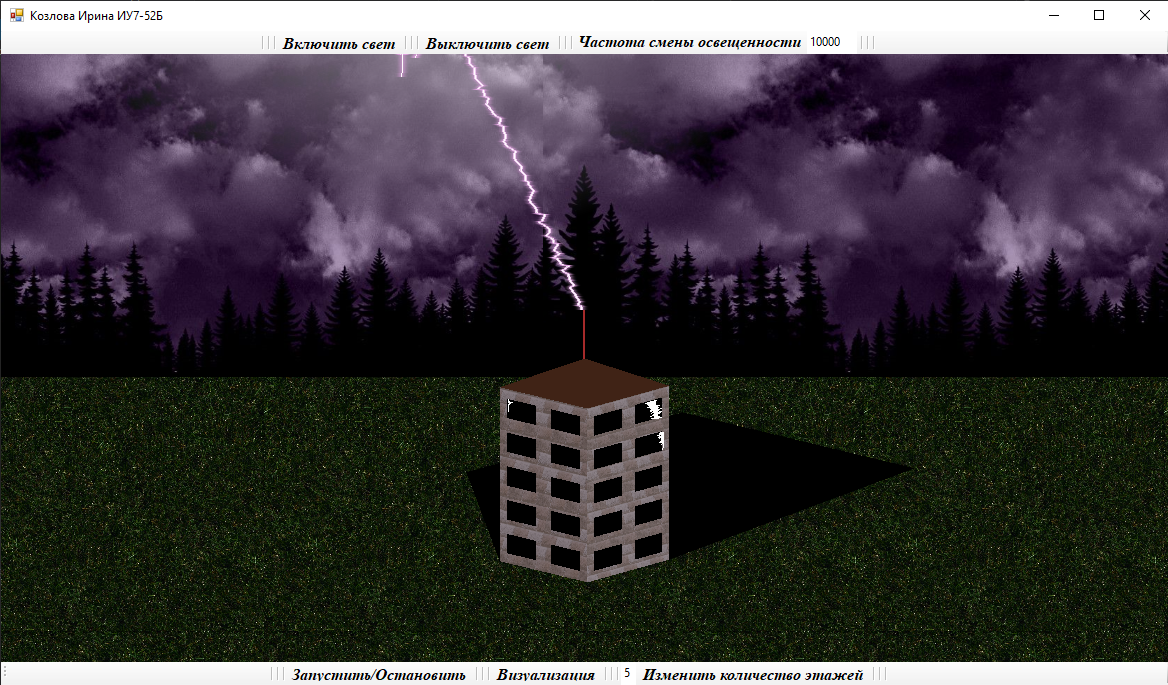
\includegraphics[scale=0.40]{img/prog_res/s1.png}
	\end{center}
	\captionsetup{justification=centering}
	\caption{Сцена 1}
	\label{img:s1}
\end{figure}

Чтобы посчитать количество лучей, с помощью которых строится сцена, необходимо посчитать количество лучей, которые испускаются в окна (равно количеству пикселей), и сложить с количеством лучей, которые пускаются во все сегменты молнии.

Количество лучей, испускаемых из всех окон, в которых выключен свет и которые ''видны'' пользователю вычисляется по формуле \ref{eq:s1}.
\begin{equation}
	\label{eq:s1}
	N * S =  20 * 800 = 16 000 лучей,
\end{equation}
где $N$ -- количество окон, в которых не горит свет и которые видны пользователю, $S$ -- размер окна в пикселях (pазмер каждого окна -- $40 * 20 = 800$).

Количество лучей, которые пускаются во все сегменты молнии равно соответственно количеству сегментов молнии, то есть около 100 сегментов на каждую ветвь. В данном примере это количество можно вычислить по формуле \ref{eq:s11}
\begin{equation}
	\label{eq:s11}
	Seg * V = 100 * 1 = 100 лучей,
\end{equation}
где $Seg$ -- количество сегментов для каждой ветви молнии, $V$ -- количество ветвей.

Суммируя найденные результаты, получается, что для того, чтобы нарисовать данную сцену потребовалось $16 000 + 100 = 16 100$ лучей.

Далее следует посчитать количество лучей, которые потребовались для визуализации сцены при использовании алгоритма обратной трассировки лучей без улучшений. 

В стандартной алгоритме требуется пустить лучи в каждый пиксель сцены. Размер сцены данной программы в пикселях -- $1139 * 632 = 719 848$, что соответствует количеству лучей, с помощью которых будет сгенерирована сцена.

Таким образом, можно сказать, что улучшенный алгоритм обратной трассировки лучей требует в $\frac{719 848}{16100} \approx 44$ раза меньше лучей для построения сцены, от чего напрямую зависит, что и времени требуется в 44 раза меньше. 

Аналогично считались количество испускаемых лучей для генерации сцены с домом разной этажностью. Свет во всех окнах выключен, а сам дом повернут на 45 градусов относительно своей оси. Молния бьет всегда в громоотвод, не имея побочных ветвей.

Подсчет лучей приведен в таблице \ref{tab:time1}.

Обозначения:
\begin{itemize}
	\item АОТЛ -- алгоритм обратной трассировки лучей;
	\item ОАОТЛ -- оптимизированный алгоритм трассировки лучей.
	\item Улучшение -- во сколько раз оптимизированный алгоритм испускает лучей меньше, чем простой.
\end{itemize}

\begin{table}[h]
	\begin{center}
		\caption{\label{tab:time1}Количество лучей для генерации сцены}
		\begin{tabular}{|c|c|c|c|c|}
			\hline
			Количество этажей & АОТЛ &  ОАОТЛ & Улучшение \\
			\hline
			1  & 719 848 & 3300 & 218 \\
			\hline
			2  & 719 848 & 6500 & 110 \\
			\hline
			3  & 719 848 & 9700 & 74 \\
			\hline
			4  & 719 848 & 12900 & 55 \\
			\hline
			5  & 719 848 & 16100 & 44 \\
			\hline
			6  & 719 848 & 19300 & 37 \\
			\hline
			7  & 719 848 & 22500 & 31 \\
			\hline
			8  & 719 848 & 25700 &  28 \\
			\hline
			9  & 719 848 & 28900 & 25 \\
			\hline
			
		\end{tabular}
	\end{center}
\end{table}


\section{Программный расчет}
Расчитанные выше значения были подтверждены программно.

На рисунке \ref{img:e4} приведен график зависимости количества лучей от количества этажей.

Синий график -- количество лучей, подсчитанных аналитическим способом. 

Оранжевый график -- количесво лучей, подсчитанных программным способом.

\begin{figure}[H]
	\begin{center}
		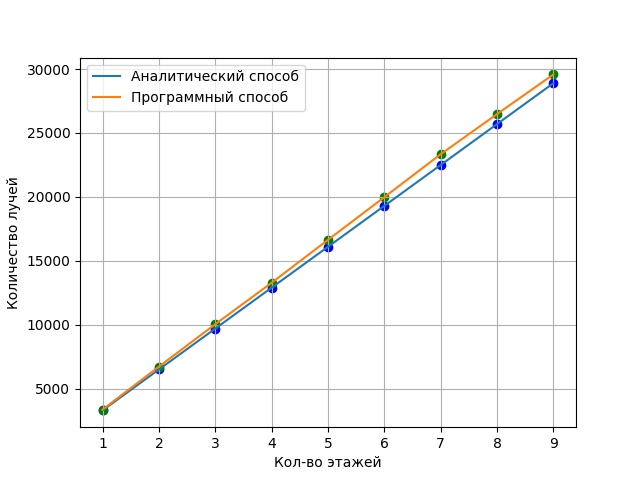
\includegraphics[scale=0.80]{img/res/e4.png}
	\end{center}
	\captionsetup{justification=centering}
	\caption{Количество лучей (количество этажей)}
	\label{img:e4}
\end{figure}



\section{Вывод}

В результате эксперимента было выявлено, что оптимизированный алгоритм обратной трассировки лучей на самом деле дает выигрыш во времени, так как требует меньшего количества лучей для построения сцены. Кроме того, расчитанные аналитическим способом результаты были подтверждены на практике.

